\documentclass{standalone}
\usepackage{tikz}
\usetikzlibrary{patterns, positioning}
\usepackage[sfdefault]{ClearSans} %% option 'sfdefault' activates Clear Sans as the default text font
\usepackage[T1]{fontenc}

\begin{document}
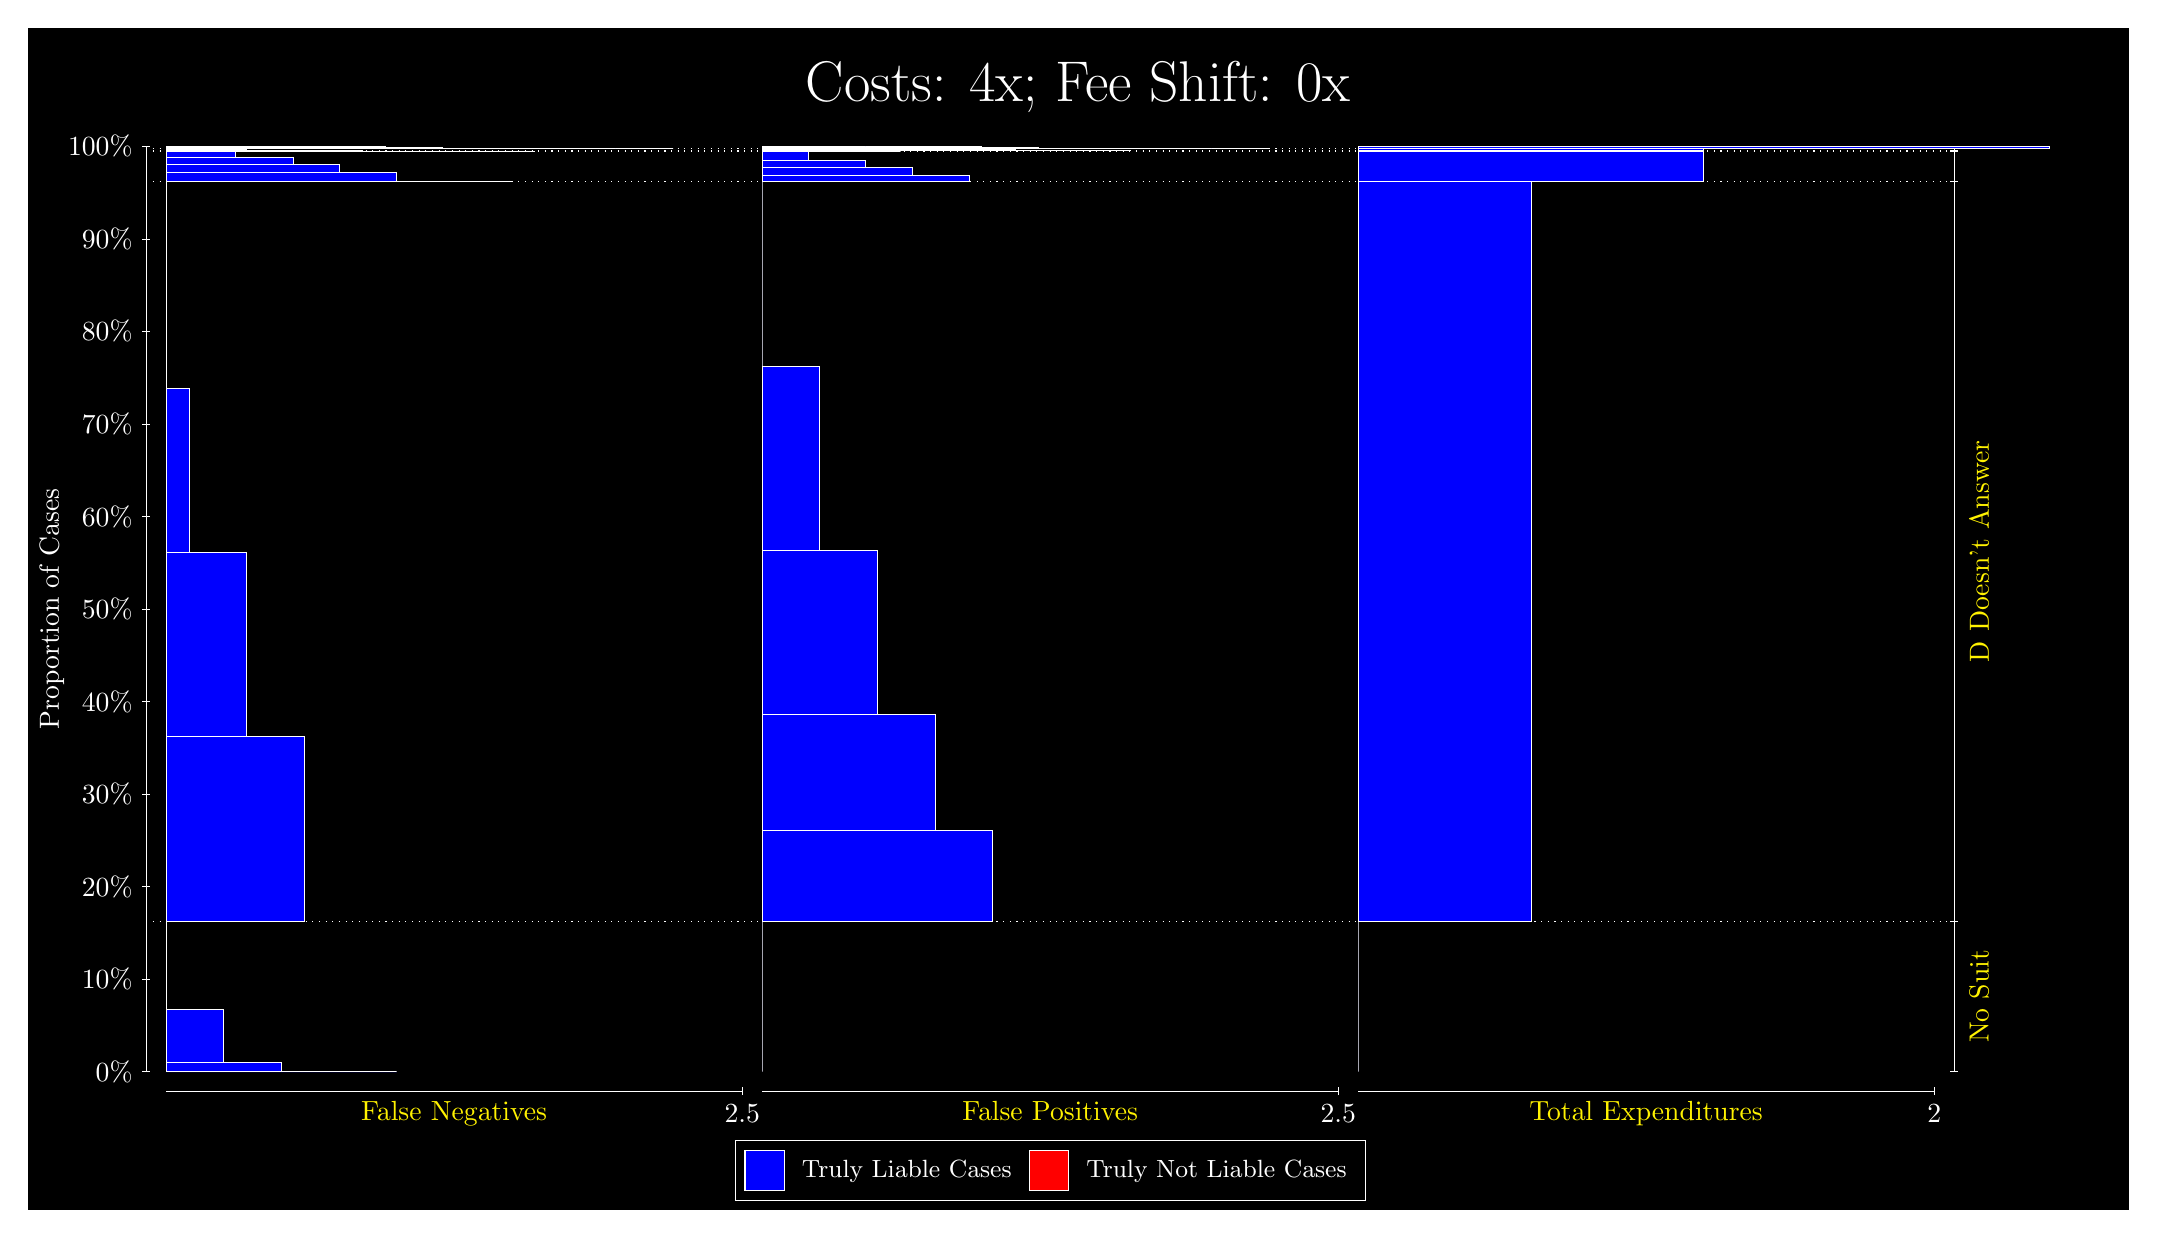
\begin{tikzpicture}
\draw[fill=black] (0,0) rectangle (26.667,15);
\draw[text=white] (0,13.5) rectangle (26.667,15) node[midway] {\huge Costs: 4x; Fee Shift: 0x};
\draw[white, very thin] (1.5,1.75) -- (1.5,13.5);
\node[rotate=90, text=white, anchor=center] at (0.3, 7.625) {Proportion of Cases};
\draw[white, very thin] (1.45,1.75) -- (1.55,1.75);
\node[text=white, anchor=east] at (1.45, 1.75) {0\%};
\draw[white, very thin] (1.45,2.925) -- (1.55,2.925);
\node[text=white, anchor=east] at (1.45, 2.925) {10\%};
\draw[white, very thin] (1.45,4.1) -- (1.55,4.1);
\node[text=white, anchor=east] at (1.45, 4.1) {20\%};
\draw[white, very thin] (1.45,5.275) -- (1.55,5.275);
\node[text=white, anchor=east] at (1.45, 5.275) {30\%};
\draw[white, very thin] (1.45,6.45) -- (1.55,6.45);
\node[text=white, anchor=east] at (1.45, 6.45) {40\%};
\draw[white, very thin] (1.45,7.625) -- (1.55,7.625);
\node[text=white, anchor=east] at (1.45, 7.625) {50\%};
\draw[white, very thin] (1.45,8.8) -- (1.55,8.8);
\node[text=white, anchor=east] at (1.45, 8.8) {60\%};
\draw[white, very thin] (1.45,9.975) -- (1.55,9.975);
\node[text=white, anchor=east] at (1.45, 9.975) {70\%};
\draw[white, very thin] (1.45,11.15) -- (1.55,11.15);
\node[text=white, anchor=east] at (1.45, 11.15) {80\%};
\draw[white, very thin] (1.45,12.325) -- (1.55,12.325);
\node[text=white, anchor=east] at (1.45, 12.325) {90\%};
\draw[white, very thin] (1.45,13.5) -- (1.55,13.5);
\node[text=white, anchor=east] at (1.45, 13.5) {100\%};

\draw[white, very thin] (24.457,1.75) -- (24.457,13.5);
\draw[white, very thin] (24.407,1.75) -- (24.507,1.75);
\node[anchor=west] at (24.407, 1.75) {};
\draw[white, very thin] (24.407,3.6576) -- (24.507,3.6576);
\node[anchor=west] at (24.407, 3.6576) {};
\draw[white, very thin] (24.407,13.057) -- (24.507,13.057);
\node[anchor=west] at (24.407, 13.057) {};
\draw[white, very thin] (24.407,13.439) -- (24.507,13.439);
\node[anchor=west] at (24.407, 13.439) {};
\draw[white, very thin] (24.407,13.448) -- (24.507,13.448);
\node[anchor=west] at (24.407, 13.448) {};
\draw[white, very thin] (24.407,13.475) -- (24.507,13.475);
\node[anchor=west] at (24.407, 13.475) {};
\draw[white, very thin] (24.407,13.5) -- (24.507,13.5);
\node[anchor=west] at (24.407, 13.5) {};

\draw[white, very thin, fill=blue] (1.75,1.75) rectangle (4.6775,1.75);
\draw[white, very thin, fill=blue] (1.75,1.75) rectangle (3.9457,1.751);
\draw[white, very thin, fill=blue] (1.75,1.751) rectangle (3.2138,1.8646);
\draw[white, very thin, fill=blue] (1.75,1.8646) rectangle (2.4819,2.5421);
\draw[white, very thin, fill=red] (1.75,2.5421) rectangle (1.75,2.5421);
\draw[white, very thin, fill=blue] (1.75,2.5421) rectangle (1.75,3.6576);
\draw[white, very thin, fill=blue] (1.75,3.6576) rectangle (3.5065,6.0074);
\draw[white, very thin, fill=blue] (1.75,6.0074) rectangle (2.7746,8.3422);
\draw[white, very thin, fill=blue] (1.75,8.3422) rectangle (2.0428,10.426);
\draw[white, very thin, fill=red] (1.75,10.426) rectangle (1.75,10.426);
\draw[white, very thin, fill=blue] (1.75,10.426) rectangle (1.75,13.057);
\draw[white, very thin, fill=blue] (1.75,13.057) rectangle (6.1413,13.057);
\draw[white, very thin, fill=blue] (1.75,13.057) rectangle (5.5558,13.057);
\draw[white, very thin, fill=blue] (1.75,13.057) rectangle (5.4094,13.059);
\draw[white, very thin, fill=blue] (1.75,13.059) rectangle (4.8239,13.059);
\draw[white, very thin, fill=blue] (1.75,13.059) rectangle (4.6775,13.17);
\draw[white, very thin, fill=blue] (1.75,13.17) rectangle (4.092,13.176);
\draw[white, very thin, fill=blue] (1.75,13.176) rectangle (3.9457,13.268);
\draw[white, very thin, fill=blue] (1.75,13.268) rectangle (3.3602,13.36);
\draw[white, very thin, fill=blue] (1.75,13.36) rectangle (3.2138,13.361);
\draw[white, very thin, fill=blue] (1.75,13.361) rectangle (2.6283,13.439);
\draw[white, very thin, fill=red] (1.75,13.439) rectangle (1.75,13.439);
\draw[white, very thin, fill=blue] (1.75,13.439) rectangle (6.4341,13.439);
\draw[white, very thin, fill=blue] (1.75,13.439) rectangle (5.7022,13.439);
\draw[white, very thin, fill=blue] (1.75,13.439) rectangle (4.9703,13.443);
\draw[white, very thin, fill=blue] (1.75,13.443) rectangle (4.2384,13.447);
\draw[white, very thin, fill=blue] (1.75,13.447) rectangle (3.5065,13.448);
\draw[white, very thin, fill=red] (1.75,13.448) rectangle (1.75,13.448);
\draw[white, very thin, fill=blue] (1.75,13.448) rectangle (3.5065,13.448);
\draw[white, very thin, fill=blue] (1.75,13.448) rectangle (2.7746,13.459);
\draw[white, very thin, fill=blue] (1.75,13.459) rectangle (2.0428,13.473);
\draw[white, very thin, fill=red] (1.75,13.473) rectangle (1.75,13.473);
\draw[white, very thin, fill=blue] (1.75,13.473) rectangle (1.75,13.475);
\draw[white, very thin, fill=blue] (1.75,13.475) rectangle (8.1906,13.475);
\draw[white, very thin, fill=blue] (1.75,13.475) rectangle (7.4587,13.475);
\draw[white, very thin, fill=blue] (1.75,13.475) rectangle (6.7268,13.475);
\draw[white, very thin, fill=blue] (1.75,13.475) rectangle (5.9949,13.481);
\draw[white, very thin, fill=blue] (1.75,13.481) rectangle (5.2631,13.494);
\draw[white, very thin, fill=blue] (1.75,13.494) rectangle (4.5312,13.499);
\draw[white, very thin, fill=blue] (1.75,13.499) rectangle (3.7993,13.5);
\draw[white, very thin, fill=blue] (1.75,13.5) rectangle (3.0674,13.5);
\draw[white, very thin, fill=blue] (1.75,13.5) rectangle (2.3355,13.5);
\draw[white, very thin, fill=red] (1.75,13.5) rectangle (1.75,13.5);
\draw[white, very thin, fill=red] (9.3189,1.75) rectangle (9.3189,1.75);
\draw[white, very thin, fill=blue] (9.3189,1.75) rectangle (9.3189,3.6576);
\draw[white, very thin, fill=red] (9.3189,3.6576) rectangle (12.246,3.6576);
\draw[white, very thin, fill=blue] (9.3189,3.6576) rectangle (12.246,4.8127);
\draw[white, very thin, fill=blue] (9.3189,4.8127) rectangle (11.515,6.289);
\draw[white, very thin, fill=blue] (9.3189,6.289) rectangle (10.783,8.3726);
\draw[white, very thin, fill=blue] (9.3189,8.3726) rectangle (10.051,10.707);
\draw[white, very thin, fill=blue] (9.3189,10.707) rectangle (9.3189,13.057);
\draw[white, very thin, fill=red] (9.3189,13.057) rectangle (11.954,13.057);
\draw[white, very thin, fill=blue] (9.3189,13.057) rectangle (11.954,13.135);
\draw[white, very thin, fill=red] (9.3189,13.135) rectangle (11.368,13.135);
\draw[white, very thin, fill=blue] (9.3189,13.135) rectangle (11.368,13.136);
\draw[white, very thin, fill=blue] (9.3189,13.136) rectangle (11.222,13.228);
\draw[white, very thin, fill=blue] (9.3189,13.228) rectangle (10.636,13.32);
\draw[white, very thin, fill=blue] (9.3189,13.32) rectangle (10.49,13.326);
\draw[white, very thin, fill=blue] (9.3189,13.326) rectangle (9.9044,13.437);
\draw[white, very thin, fill=blue] (9.3189,13.437) rectangle (9.758,13.437);
\draw[white, very thin, fill=blue] (9.3189,13.437) rectangle (9.3189,13.439);
\draw[white, very thin, fill=red] (9.3189,13.439) rectangle (11.075,13.439);
\draw[white, very thin, fill=blue] (9.3189,13.439) rectangle (11.075,13.439);
\draw[white, very thin, fill=blue] (9.3189,13.439) rectangle (10.344,13.443);
\draw[white, very thin, fill=blue] (9.3189,13.443) rectangle (9.6116,13.447);
\draw[white, very thin, fill=blue] (9.3189,13.447) rectangle (9.3189,13.448);
\draw[white, very thin, fill=red] (9.3189,13.448) rectangle (14.003,13.448);
\draw[white, very thin, fill=blue] (9.3189,13.448) rectangle (14.003,13.448);
\draw[white, very thin, fill=blue] (9.3189,13.448) rectangle (13.271,13.45);
\draw[white, very thin, fill=blue] (9.3189,13.45) rectangle (12.539,13.464);
\draw[white, very thin, fill=blue] (9.3189,13.464) rectangle (11.807,13.475);
\draw[white, very thin, fill=blue] (9.3189,13.475) rectangle (11.075,13.475);
\draw[white, very thin, fill=red] (9.3189,13.475) rectangle (15.759,13.475);
\draw[white, very thin, fill=blue] (9.3189,13.475) rectangle (15.759,13.475);
\draw[white, very thin, fill=blue] (9.3189,13.475) rectangle (15.028,13.475);
\draw[white, very thin, fill=red] (9.3189,13.475) rectangle (15.028,13.475);
\draw[white, very thin, fill=blue] (9.3189,13.475) rectangle (15.028,13.475);
\draw[white, very thin, fill=blue] (9.3189,13.475) rectangle (14.296,13.475);
\draw[white, very thin, fill=red] (9.3189,13.475) rectangle (14.296,13.475);
\draw[white, very thin, fill=blue] (9.3189,13.475) rectangle (14.296,13.476);
\draw[white, very thin, fill=blue] (9.3189,13.476) rectangle (13.564,13.476);
\draw[white, very thin, fill=red] (9.3189,13.476) rectangle (13.564,13.476);
\draw[white, very thin, fill=blue] (9.3189,13.476) rectangle (13.564,13.481);
\draw[white, very thin, fill=blue] (9.3189,13.481) rectangle (12.832,13.481);
\draw[white, very thin, fill=red] (9.3189,13.481) rectangle (12.832,13.481);
\draw[white, very thin, fill=blue] (9.3189,13.481) rectangle (12.832,13.494);
\draw[white, very thin, fill=blue] (9.3189,13.494) rectangle (12.1,13.5);
\draw[white, very thin, fill=blue] (9.3189,13.5) rectangle (11.368,13.5);
\draw[white, very thin, fill=blue] (9.3189,13.5) rectangle (10.636,13.5);
\draw[white, very thin, fill=blue] (9.3189,13.5) rectangle (9.9044,13.5);
\draw[white, very thin, fill=red] (16.888,1.75) rectangle (16.888,1.75);
\draw[white, very thin, fill=blue] (16.888,1.75) rectangle (16.888,3.6576);
\draw[white, very thin, fill=red] (16.888,3.6576) rectangle (19.083,3.6576);
\draw[white, very thin, fill=blue] (16.888,3.6576) rectangle (19.083,13.057);
\draw[white, very thin, fill=red] (16.888,13.057) rectangle (21.279,13.057);
\draw[white, very thin, fill=blue] (16.888,13.057) rectangle (21.279,13.439);
\draw[white, very thin, fill=red] (16.888,13.439) rectangle (21.279,13.439);
\draw[white, very thin, fill=blue] (16.888,13.439) rectangle (21.279,13.448);
\draw[white, very thin, fill=red] (16.888,13.448) rectangle (21.279,13.448);
\draw[white, very thin, fill=blue] (16.888,13.448) rectangle (21.279,13.475);
\draw[white, very thin, fill=red] (16.888,13.475) rectangle (25.67,13.475);
\draw[white, very thin, fill=blue] (16.888,13.475) rectangle (25.67,13.476);
\draw[white, very thin, fill=red] (16.888,13.476) rectangle (25.67,13.476);
\draw[white, very thin, fill=blue] (16.888,13.476) rectangle (25.67,13.5);
\draw[white, dotted] (1.5,3.6576) -- (24.457,3.6576);
\draw[white, dotted] (1.5,13.057) -- (24.457,13.057);
\draw[white, dotted] (1.5,13.439) -- (24.457,13.439);
\draw[white, dotted] (1.5,13.448) -- (24.457,13.448);
\draw[white, dotted] (1.5,13.475) -- (24.457,13.475);
\draw[white, very thin] (1.75,1.5) -- (9.0689,1.5);
\node[text=yellow, anchor=north] at (5.4094, 1.5) {False Negatives};
\draw[white, very thin] (9.0689,1.45) -- (9.0689,1.55);
\node[text=white, anchor=north] at (9.0689, 1.45) {2.5};

\draw[white, very thin] (9.3189,1.5) -- (16.638,1.5);
\node[text=yellow, anchor=north] at (12.978, 1.5) {False Positives};
\draw[white, very thin] (16.638,1.45) -- (16.638,1.55);
\node[text=white, anchor=north] at (16.638, 1.45) {2.5};

\draw[white, very thin] (16.888,1.5) -- (24.207,1.5);
\node[text=yellow, anchor=north] at (20.547, 1.5) {Total Expenditures};
\draw[white, very thin] (24.207,1.45) -- (24.207,1.55);
\node[text=white, anchor=north] at (24.207, 1.45) {2};

\node[text=yellow, centered, rotate=90] at (24.777, 2.7038) {No Suit};
\node[text=yellow, centered, rotate=90] at (24.777, 8.3574) {D Doesn't Answer};





\draw (12.978300999999998,1.5) node[draw=none] (baseCoordinate) {};
\begin{scope}[align=center]
        \matrix[scale=0.5, draw=white, below=0.5cm of baseCoordinate, nodes={draw}, column sep=0.1cm]{
            \node[rectangle, draw, minimum width=0.5cm, minimum height=0.5cm, fill=blue] {}; &
            \node[draw=none, font=\small, text=white] (B) {Truly Liable Cases}; &
            \node[rectangle, draw, minimum width=0.5cm, minimum height=0.5cm, fill=red] {}; &
            \node[draw=none, font=\small, text=white] (B) {Truly Not Liable Cases}; \\
            };
\end{scope}

\end{tikzpicture}
\end{document}